\documentclass{standalone}
\usepackage{tikz}
\usepackage{amssymb}
\usepackage{amsmath}
\usepackage{amstext}
\usepackage{xcolor}
\usetikzlibrary{positioning,shapes.geometric}
\usetikzlibrary{arrows}
\begin{document}

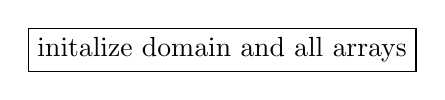
\begin{tikzpicture}[
	  scale=1.0,
	  %style for arrows
	  arrw/.style={thick, ->, >=to},
      % fisrt style for boxes      
      op/.style={rectangle, fill=black!15, draw=black},
      % second style for boxes
      dt/.style={rectangle, fill=white, draw=black}]
            
      \node[dt](initdom){initalize domain and all arrays};
    

\end{tikzpicture}
  
\end{document}